\documentclass{article}

% packages
\usepackage{ctex}
\usepackage{amsmath}
\usepackage{amsthm}
\usepackage{graphicx}

\title{直径规约整理}
\author{}
\date{}

\begin{document}
\maketitle

\section{计算上界$U$}
我们可以通过计算具有$n$个点的$k$-defective的直径$d$的上界来
对我们原来的问题进行简化. 这篇文章将计算这个上界的思路进行整理.

为了方便计算, 我们首先需要将图进行转化.
假设我们有一个图,$G = (V, E)$. 这个图是一个$k$-defective.
其中$s, t \in V$两个点之间的一条路径是$G$的一个直径, 这条直径的长度为$d$.

通过将整个图$G$中的点按照到$s$的距离进行分层, 可以将原来的图绘制成一个分层图,
其中$s$在第$0$层, $t$在第$d$层 (示意图见图\ref{fig:1}). 

画好分层图之后, 可以将图中的边分为两种, 一种是一个端点在直径上的边(蓝色), 另外一种是
两个端点都不在直径上的边(红色).

\begin{figure}[h!]
	\begin{center}
		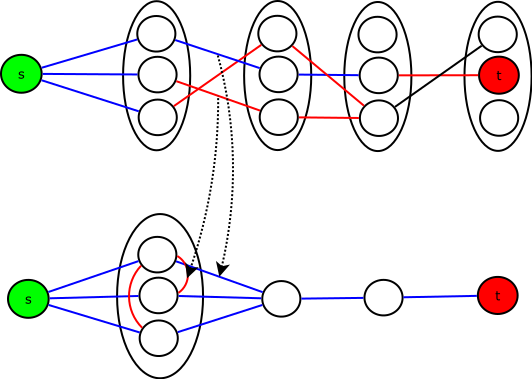
\includegraphics[width=8cm]{origin-to-special.png} \\
		\caption{转换方式示意图}
		\label{fig:1}
	\end{center}
\end{figure}

通过将所有其他层中不在直径上的点移动到第一层, 我们可以得到如图\ref{fig:1}所示的新图.
这张图与原图的点数和边数是一样的(虽然没有画得一样).

我们可以在第一层中补充新的边, 将第一层补充成一个团, 这样, 可以得到关于边数$|E|$的一个上界$M$.
即$M \geq |E|$. 再结合$k$-defective的定义$|E| \geq \left(\begin{array}{c} n \\ 2 \end{array}\right) - k$.
最终我们可以得到: $M \geq \left(\begin{array}{c} n \\ 2 \end{array}\right) - k$.
根据上面的图\ref{fig:1}, 我们可以将$M$展开成如下形式:
\[
	M = 
	\left( \begin{array}{c}
		n -d \\ 2
	\end{array} \right)
   	+ 2(n-d) + (d-2)
\]
综合上面的式子可以得到关于$d$的约束:
\[
	\left( \begin{array}{c}
		n -d \\ 2
	\end{array} \right)
   	+ 2(n-d) + (d-2)
	\geq
	\left(\begin{array}{c} n \\ 2 \end{array}\right) - k
\]
解这个式子可以得到:
\[
	\left\{
		\begin{array}{l}
			d \leq \frac{(2n+1) - \sqrt{4n^2 - 12n + 17 - 8k}}{2} \\
			d \geq \frac{(2n+1) + \sqrt{4n^2 - 12n + 17 - 8k}}{2} (\mbox{不可能发生, 因为$d \leq n-1$}) \\
		\end{array}
	\right.
\]
故, 最终可以得到: $d \leq \frac{(2n+1) - \sqrt{4n^2 - 12n + 17 - 8k}}{2} = U$.
并且我们可以知道: 只要$\Delta = 4n^2 - 12n + 17 - 8k \geq 0$, 这个上界就是有效的.

总结一下, $U$是: 有$n$个点的$k$-defective的直径长度的上界.

\section{在分支中使用上界$U^*$}
上界$U$是不能直接在分支的时候使用的, 因为$U$是一个和$n$有关的函数$U(n)$
($k$一旦给定就不会变, 这里可以看成常数), 其中$n$是$k$-defective中的点数.
假设最优解的大小为$x$, 则最优解中直径的上界为$U(x)$. 因为我们不知道$x$, 
所以, 实际上我们不能直接使用$U(x)$.

但是, 观察$U(n)$的图像(图\ref{fig:2}, 图\ref{fig:3}), 
我们可以猜想:
$\exists l \geq 0$ 使得当 $n > l$ 时, $U(n) \leq U(l)$.
如果是这样的话, 则我们可以令$U^* = U(l) \geq U(n) \geq |E|$作为分支时使用的上界.

\begin{figure}[h!]
	\begin{center}
		\includegraphics[width=12cm]{function-1.png} \\
		\caption{$k = 1$时, 上界的图像}
		\label{fig:2}
	\end{center}
\end{figure}

\begin{figure}[h!]
	\begin{center}
		\includegraphics[width=12cm]{function-g1.png} \\
		\caption{$k > 1$时, 上界的图像}
		\label{fig:3}
	\end{center}
\end{figure}

令$U(n) = \frac{(2n+1) - \sqrt{4n^2 - 12n + 17 - 8k}}{2}$.
则:
\[
	U'(n) = 1 - \frac{2n-3}{\sqrt{4n^2 - 12n + 17 - 8k}}
\]
继续化简一下可以得:
\[
	U'(n) = 1 - sgn(2n-3)\sqrt{\frac{4n^2 - 12n + 17 - 8}{4n^2 - 12n + 17 - 8k}}
\]
故当$2n-3 \geq 0$时:\\
当$k = 1$, 且$\Delta = 4n^2 - 12n + 17 - 8k \geq 0$时, $U'(n) = 1$.\\
当$k > 1$, 且$\Delta = 4n^2 - 12n + 17 - 8k \geq 0$时, $U'(n) < 1$单调递减. \\
这就证明了之前的猜想的正确性.

总结一下: 假设我们现在得到了最优解的下界$l$, 
且满足如下条件
\[
	\left\{
		\begin{array}{l}
			k \geq 1 \\
			\Delta = 4l^2 - 12l + 17 - 8k > 0\\
			2l - 3 \geq 0
		\end{array}
	\right.
\]
则我们可以得到一个最优解的直径的上界$U^* = U(l)$.

\end{document}
